\documentclass[twoside]{book}

% Packages required by doxygen
\usepackage{fixltx2e}
\usepackage{calc}
\usepackage{doxygen}
\usepackage[export]{adjustbox} % also loads graphicx
\usepackage{graphicx}
\usepackage[utf8]{inputenc}
\usepackage{makeidx}
\usepackage{multicol}
\usepackage{multirow}
\PassOptionsToPackage{warn}{textcomp}
\usepackage{textcomp}
\usepackage[nointegrals]{wasysym}
\usepackage[table]{xcolor}

% Font selection
\usepackage[T1]{fontenc}
\usepackage[scaled=.90]{helvet}
\usepackage{courier}
\usepackage{amssymb}
\usepackage{sectsty}
\renewcommand{\familydefault}{\sfdefault}
\allsectionsfont{%
  \fontseries{bc}\selectfont%
  \color{darkgray}%
}
\renewcommand{\DoxyLabelFont}{%
  \fontseries{bc}\selectfont%
  \color{darkgray}%
}
\newcommand{\+}{\discretionary{\mbox{\scriptsize$\hookleftarrow$}}{}{}}

% Page & text layout
\usepackage{geometry}
\geometry{%
  a4paper,%
  top=2.5cm,%
  bottom=2.5cm,%
  left=2.5cm,%
  right=2.5cm%
}
\tolerance=750
\hfuzz=15pt
\hbadness=750
\setlength{\emergencystretch}{15pt}
\setlength{\parindent}{0cm}
\setlength{\parskip}{3ex plus 2ex minus 2ex}
\makeatletter
\renewcommand{\paragraph}{%
  \@startsection{paragraph}{4}{0ex}{-1.0ex}{1.0ex}{%
    \normalfont\normalsize\bfseries\SS@parafont%
  }%
}
\renewcommand{\subparagraph}{%
  \@startsection{subparagraph}{5}{0ex}{-1.0ex}{1.0ex}{%
    \normalfont\normalsize\bfseries\SS@subparafont%
  }%
}
\makeatother

% Headers & footers
\usepackage{fancyhdr}
\pagestyle{fancyplain}
\fancyhead[LE]{\fancyplain{}{\bfseries\thepage}}
\fancyhead[CE]{\fancyplain{}{}}
\fancyhead[RE]{\fancyplain{}{\bfseries\leftmark}}
\fancyhead[LO]{\fancyplain{}{\bfseries\rightmark}}
\fancyhead[CO]{\fancyplain{}{}}
\fancyhead[RO]{\fancyplain{}{\bfseries\thepage}}
\fancyfoot[LE]{\fancyplain{}{}}
\fancyfoot[CE]{\fancyplain{}{}}
\fancyfoot[RE]{\fancyplain{}{\bfseries\scriptsize Generated by Doxygen }}
\fancyfoot[LO]{\fancyplain{}{\bfseries\scriptsize Generated by Doxygen }}
\fancyfoot[CO]{\fancyplain{}{}}
\fancyfoot[RO]{\fancyplain{}{}}
\renewcommand{\footrulewidth}{0.4pt}
\renewcommand{\chaptermark}[1]{%
  \markboth{#1}{}%
}
\renewcommand{\sectionmark}[1]{%
  \markright{\thesection\ #1}%
}

% Indices & bibliography
\usepackage{natbib}
\usepackage[titles]{tocloft}
\setcounter{tocdepth}{3}
\setcounter{secnumdepth}{5}
\makeindex

% Hyperlinks (required, but should be loaded last)
\usepackage{ifpdf}
\ifpdf
  \usepackage[pdftex,pagebackref=true]{hyperref}
\else
  \usepackage[ps2pdf,pagebackref=true]{hyperref}
\fi
\hypersetup{%
  colorlinks=true,%
  linkcolor=blue,%
  citecolor=blue,%
  unicode%
}

% Custom commands
\newcommand{\clearemptydoublepage}{%
  \newpage{\pagestyle{empty}\cleardoublepage}%
}

\usepackage{caption}
\captionsetup{labelsep=space,justification=centering,font={bf},singlelinecheck=off,skip=4pt,position=top}

%===== C O N T E N T S =====

\begin{document}

% Titlepage & ToC
\hypersetup{pageanchor=false,
             bookmarksnumbered=true,
             pdfencoding=unicode
            }
\pagenumbering{roman}
\begin{titlepage}
\vspace*{7cm}
\begin{center}%
{\Large My Project }\\
\vspace*{1cm}
{\large Generated by Doxygen 1.8.11}\\
\end{center}
\end{titlepage}
\clearemptydoublepage
\tableofcontents
\clearemptydoublepage
\pagenumbering{arabic}
\hypersetup{pageanchor=true}

%--- Begin generated contents ---
\chapter{Class Index}
\section{Class List}
Here are the classes, structs, unions and interfaces with brief descriptions\+:\begin{DoxyCompactList}
\item\contentsline{section}{\hyperlink{structnode}{node} }{\pageref{structnode}}{}
\item\contentsline{section}{\hyperlink{structnode1}{node1} }{\pageref{structnode1}}{}
\item\contentsline{section}{\hyperlink{structnode__info}{node\+\_\+info} }{\pageref{structnode__info}}{}
\end{DoxyCompactList}

\chapter{File Index}
\section{File List}
Here is a list of all files with brief descriptions\+:\begin{DoxyCompactList}
\item\contentsline{section}{\hyperlink{Lab1_8c}{Lab1.\+c} }{\pageref{Lab1_8c}}{}
\end{DoxyCompactList}

\chapter{Class Documentation}
\hypertarget{structbtnode}{}\section{btnode Struct Reference}
\label{structbtnode}\index{btnode@{btnode}}


Collaboration diagram for btnode\+:
\nopagebreak
\begin{figure}[H]
\begin{center}
\leavevmode
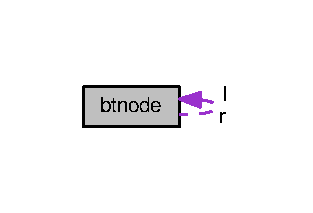
\includegraphics[width=150pt]{structbtnode__coll__graph}
\end{center}
\end{figure}
\subsection*{Public Attributes}
\begin{DoxyCompactItemize}
\item 
int \hyperlink{structbtnode_a616f93e36ddf887708b73f6e74cd753e}{value}
\item 
struct \hyperlink{structbtnode}{btnode} $\ast$ \hyperlink{structbtnode_abe62c9ae71ac473ea157e9c6a63f84af}{r}
\item 
struct \hyperlink{structbtnode}{btnode} $\ast$ \hyperlink{structbtnode_aa602dd488fab26c3123e4a448dcd1b8d}{l}
\end{DoxyCompactItemize}


\subsection{Member Data Documentation}
\index{btnode@{btnode}!l@{l}}
\index{l@{l}!btnode@{btnode}}
\subsubsection[{\texorpdfstring{l}{l}}]{\setlength{\rightskip}{0pt plus 5cm}struct {\bf btnode} $\ast$ btnode\+::l}\hypertarget{structbtnode_aa602dd488fab26c3123e4a448dcd1b8d}{}\label{structbtnode_aa602dd488fab26c3123e4a448dcd1b8d}
\index{btnode@{btnode}!r@{r}}
\index{r@{r}!btnode@{btnode}}
\subsubsection[{\texorpdfstring{r}{r}}]{\setlength{\rightskip}{0pt plus 5cm}struct {\bf btnode}$\ast$ btnode\+::r}\hypertarget{structbtnode_abe62c9ae71ac473ea157e9c6a63f84af}{}\label{structbtnode_abe62c9ae71ac473ea157e9c6a63f84af}
\index{btnode@{btnode}!value@{value}}
\index{value@{value}!btnode@{btnode}}
\subsubsection[{\texorpdfstring{value}{value}}]{\setlength{\rightskip}{0pt plus 5cm}int btnode\+::value}\hypertarget{structbtnode_a616f93e36ddf887708b73f6e74cd753e}{}\label{structbtnode_a616f93e36ddf887708b73f6e74cd753e}


The documentation for this struct was generated from the following file\+:\begin{DoxyCompactItemize}
\item 
\hyperlink{Summation_8c}{Summation.\+c}\end{DoxyCompactItemize}

\chapter{File Documentation}
\hypertarget{Summation_8c}{}\section{Summation.\+c File Reference}
\label{Summation_8c}\index{Summation.\+c@{Summation.\+c}}
{\ttfamily \#include $<$stdio.\+h$>$}\\*
{\ttfamily \#include $<$stdlib.\+h$>$}\\*
Include dependency graph for Summation.\+c\+:
\nopagebreak
\begin{figure}[H]
\begin{center}
\leavevmode
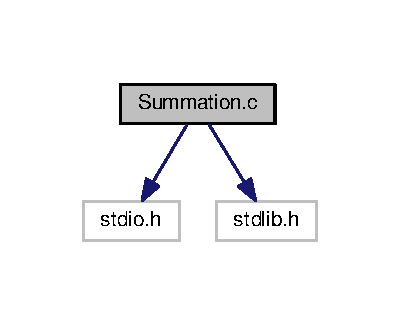
\includegraphics[width=192pt]{Summation_8c__incl}
\end{center}
\end{figure}
\subsection*{Classes}
\begin{DoxyCompactItemize}
\item 
struct \hyperlink{structbtnode}{btnode}
\end{DoxyCompactItemize}
\subsection*{Functions}
\begin{DoxyCompactItemize}
\item 
void \hyperlink{Summation_8c_ae2ee59f7cc16ee42559c87e81c433039}{create} ()
\item 
void \hyperlink{Summation_8c_a7f9d39f8cecd6bcb70ada2b9e933eb1e}{insert} ()
\item 
void \hyperlink{Summation_8c_a5c928e4b1316e80d8510f6299f396e4d}{add} (struct \hyperlink{structbtnode}{btnode} $\ast$t)
\item 
void \hyperlink{Summation_8c_a044c01529821f650d7100142d8788e6b}{computesum} (struct \hyperlink{structbtnode}{btnode} $\ast$t)
\item 
void \hyperlink{Summation_8c_a1e5b20fed15743656bb6d2e6a6ea6269}{display} ()
\item 
void \hyperlink{Summation_8c_acdef7a1fd863a6d3770c1268cb06add3}{main} ()
\end{DoxyCompactItemize}
\subsection*{Variables}
\begin{DoxyCompactItemize}
\item 
struct \hyperlink{structbtnode}{btnode} $\ast$ \hyperlink{Summation_8c_aa6fca9435ac6dc487f22b85aabd703b5}{root} = N\+U\+LL
\item 
struct \hyperlink{structbtnode}{btnode} $\ast$ \hyperlink{Summation_8c_ac0d86a861e85eeb7da1785ac8e3ae769}{temp} = N\+U\+LL
\item 
int \hyperlink{Summation_8c_ad43c3812e6d13e0518d9f8b8f463ffcf}{count} = 0
\item 
int \hyperlink{Summation_8c_abee91d89f7cb4bbc28d7949ec9d88ea8}{sum} \mbox{[}100\mbox{]} = \{0\}
\item 
int \hyperlink{Summation_8c_ae1e1dde676c120fa6d10f3bb2c14059e}{max} = 0
\end{DoxyCompactItemize}


\subsection{Function Documentation}
\index{Summation.\+c@{Summation.\+c}!add@{add}}
\index{add@{add}!Summation.\+c@{Summation.\+c}}
\subsubsection[{\texorpdfstring{add(struct btnode $\ast$t)}{add(struct btnode *t)}}]{\setlength{\rightskip}{0pt plus 5cm}void add (
\begin{DoxyParamCaption}
\item[{struct {\bf btnode} $\ast$}]{t}
\end{DoxyParamCaption}
)}\hypertarget{Summation_8c_a5c928e4b1316e80d8510f6299f396e4d}{}\label{Summation_8c_a5c928e4b1316e80d8510f6299f396e4d}

\begin{DoxyCode}
78 \{
79     \textcolor{keywordflow}{if} ((\hyperlink{Summation_8c_ac0d86a861e85eeb7da1785ac8e3ae769}{temp}->\hyperlink{structbtnode_a616f93e36ddf887708b73f6e74cd753e}{value} > t->\hyperlink{structbtnode_a616f93e36ddf887708b73f6e74cd753e}{value}) && (t->\hyperlink{structbtnode_abe62c9ae71ac473ea157e9c6a63f84af}{r} != NULL))        \textcolor{comment}{/* value more than root node
       value insert at right */}
80         \hyperlink{Summation_8c_a5c928e4b1316e80d8510f6299f396e4d}{add}(t->\hyperlink{structbtnode_abe62c9ae71ac473ea157e9c6a63f84af}{r});
81     \textcolor{keywordflow}{else} \textcolor{keywordflow}{if} ((\hyperlink{Summation_8c_ac0d86a861e85eeb7da1785ac8e3ae769}{temp}->\hyperlink{structbtnode_a616f93e36ddf887708b73f6e74cd753e}{value} > t->\hyperlink{structbtnode_a616f93e36ddf887708b73f6e74cd753e}{value}) && (t->\hyperlink{structbtnode_abe62c9ae71ac473ea157e9c6a63f84af}{r} == NULL))        
82         t->\hyperlink{structbtnode_abe62c9ae71ac473ea157e9c6a63f84af}{r} = \hyperlink{Summation_8c_ac0d86a861e85eeb7da1785ac8e3ae769}{temp};
83     \textcolor{keywordflow}{else} \textcolor{keywordflow}{if} ((\hyperlink{Summation_8c_ac0d86a861e85eeb7da1785ac8e3ae769}{temp}->\hyperlink{structbtnode_a616f93e36ddf887708b73f6e74cd753e}{value} < t->\hyperlink{structbtnode_a616f93e36ddf887708b73f6e74cd753e}{value}) && (t->\hyperlink{structbtnode_aa602dd488fab26c3123e4a448dcd1b8d}{l} != NULL))        \textcolor{comment}{/* value less than root node
       value insert at left */}
84         \hyperlink{Summation_8c_a5c928e4b1316e80d8510f6299f396e4d}{add}(t->\hyperlink{structbtnode_aa602dd488fab26c3123e4a448dcd1b8d}{l});
85     \textcolor{keywordflow}{else} \textcolor{keywordflow}{if} ((\hyperlink{Summation_8c_ac0d86a861e85eeb7da1785ac8e3ae769}{temp}->\hyperlink{structbtnode_a616f93e36ddf887708b73f6e74cd753e}{value} < t->\hyperlink{structbtnode_a616f93e36ddf887708b73f6e74cd753e}{value}) && (t->\hyperlink{structbtnode_aa602dd488fab26c3123e4a448dcd1b8d}{l}==NULL))
86         t->\hyperlink{structbtnode_aa602dd488fab26c3123e4a448dcd1b8d}{l} = \hyperlink{Summation_8c_ac0d86a861e85eeb7da1785ac8e3ae769}{temp};
87 \}
\end{DoxyCode}
\index{Summation.\+c@{Summation.\+c}!computesum@{computesum}}
\index{computesum@{computesum}!Summation.\+c@{Summation.\+c}}
\subsubsection[{\texorpdfstring{computesum(struct btnode $\ast$t)}{computesum(struct btnode *t)}}]{\setlength{\rightskip}{0pt plus 5cm}void computesum (
\begin{DoxyParamCaption}
\item[{struct {\bf btnode} $\ast$}]{t}
\end{DoxyParamCaption}
)}\hypertarget{Summation_8c_a044c01529821f650d7100142d8788e6b}{}\label{Summation_8c_a044c01529821f650d7100142d8788e6b}

\begin{DoxyCode}
91 \{
92     \textcolor{keywordflow}{if} (\hyperlink{Summation_8c_aa6fca9435ac6dc487f22b85aabd703b5}{root} == NULL)
93     \{    
94         printf(\textcolor{stringliteral}{"Tree is empty "});
95         \textcolor{keywordflow}{return};
96     \}
97     \textcolor{keywordflow}{if} (t->\hyperlink{structbtnode_aa602dd488fab26c3123e4a448dcd1b8d}{l} != NULL)
98     \{
99         \hyperlink{Summation_8c_ad43c3812e6d13e0518d9f8b8f463ffcf}{count}++;    
100         \hyperlink{Summation_8c_a044c01529821f650d7100142d8788e6b}{computesum}(t->\hyperlink{structbtnode_aa602dd488fab26c3123e4a448dcd1b8d}{l});
101     \}
102     \hyperlink{Summation_8c_abee91d89f7cb4bbc28d7949ec9d88ea8}{sum}[\hyperlink{Summation_8c_ad43c3812e6d13e0518d9f8b8f463ffcf}{count}] = \hyperlink{Summation_8c_abee91d89f7cb4bbc28d7949ec9d88ea8}{sum}[\hyperlink{Summation_8c_ad43c3812e6d13e0518d9f8b8f463ffcf}{count}] + t->\hyperlink{structbtnode_a616f93e36ddf887708b73f6e74cd753e}{value};  \textcolor{comment}{/* addition of elelment by row wise */}
103     \textcolor{keywordflow}{if} (\hyperlink{Summation_8c_ae1e1dde676c120fa6d10f3bb2c14059e}{max} < \hyperlink{Summation_8c_ad43c3812e6d13e0518d9f8b8f463ffcf}{count})
104         \hyperlink{Summation_8c_ae1e1dde676c120fa6d10f3bb2c14059e}{max} = \hyperlink{Summation_8c_ad43c3812e6d13e0518d9f8b8f463ffcf}{count};
105     \textcolor{keywordflow}{if} (t->\hyperlink{structbtnode_abe62c9ae71ac473ea157e9c6a63f84af}{r} != NULL)
106     \{
107         \hyperlink{Summation_8c_ad43c3812e6d13e0518d9f8b8f463ffcf}{count}++;        
108         \hyperlink{Summation_8c_a044c01529821f650d7100142d8788e6b}{computesum}(t->\hyperlink{structbtnode_abe62c9ae71ac473ea157e9c6a63f84af}{r});
109     \}
110     \hyperlink{Summation_8c_ad43c3812e6d13e0518d9f8b8f463ffcf}{count}--;
111 \}
\end{DoxyCode}
\index{Summation.\+c@{Summation.\+c}!create@{create}}
\index{create@{create}!Summation.\+c@{Summation.\+c}}
\subsubsection[{\texorpdfstring{create()}{create()}}]{\setlength{\rightskip}{0pt plus 5cm}void create (
\begin{DoxyParamCaption}
{}
\end{DoxyParamCaption}
)}\hypertarget{Summation_8c_ae2ee59f7cc16ee42559c87e81c433039}{}\label{Summation_8c_ae2ee59f7cc16ee42559c87e81c433039}

\begin{DoxyCode}
55 \{
56     \textcolor{keywordtype}{int} data;
57  
58     printf(\textcolor{stringliteral}{"Enter the data of node : "});
59     scanf(\textcolor{stringliteral}{"%d"}, &data);
60     \hyperlink{Summation_8c_ac0d86a861e85eeb7da1785ac8e3ae769}{temp} = (\textcolor{keyword}{struct }\hyperlink{structbtnode}{btnode}* ) malloc(1*(\textcolor{keyword}{sizeof}(\textcolor{keyword}{struct} \hyperlink{structbtnode}{btnode})));
61     \hyperlink{Summation_8c_ac0d86a861e85eeb7da1785ac8e3ae769}{temp}->\hyperlink{structbtnode_a616f93e36ddf887708b73f6e74cd753e}{value} = data;
62     \hyperlink{Summation_8c_ac0d86a861e85eeb7da1785ac8e3ae769}{temp}->\hyperlink{structbtnode_aa602dd488fab26c3123e4a448dcd1b8d}{l} = \hyperlink{Summation_8c_ac0d86a861e85eeb7da1785ac8e3ae769}{temp}->\hyperlink{structbtnode_abe62c9ae71ac473ea157e9c6a63f84af}{r} = NULL;
63 \}
\end{DoxyCode}
\index{Summation.\+c@{Summation.\+c}!display@{display}}
\index{display@{display}!Summation.\+c@{Summation.\+c}}
\subsubsection[{\texorpdfstring{display()}{display()}}]{\setlength{\rightskip}{0pt plus 5cm}void display (
\begin{DoxyParamCaption}
{}
\end{DoxyParamCaption}
)}\hypertarget{Summation_8c_a1e5b20fed15743656bb6d2e6a6ea6269}{}\label{Summation_8c_a1e5b20fed15743656bb6d2e6a6ea6269}

\begin{DoxyCode}
115 \{
116     \textcolor{keywordtype}{int} i;
117  
118     printf(\textcolor{stringliteral}{"Sum of nodes : \(\backslash\)n Level \(\backslash\)t Sum "});
119     \textcolor{keywordflow}{for} (i = 0; i <= \hyperlink{Summation_8c_ae1e1dde676c120fa6d10f3bb2c14059e}{max}; i++)
120        printf(\textcolor{stringliteral}{"\(\backslash\)n %d \(\backslash\)t: %d "}, i, \hyperlink{Summation_8c_abee91d89f7cb4bbc28d7949ec9d88ea8}{sum}[i]);
121 \}\end{DoxyCode}
\index{Summation.\+c@{Summation.\+c}!insert@{insert}}
\index{insert@{insert}!Summation.\+c@{Summation.\+c}}
\subsubsection[{\texorpdfstring{insert()}{insert()}}]{\setlength{\rightskip}{0pt plus 5cm}void insert (
\begin{DoxyParamCaption}
{}
\end{DoxyParamCaption}
)}\hypertarget{Summation_8c_a7f9d39f8cecd6bcb70ada2b9e933eb1e}{}\label{Summation_8c_a7f9d39f8cecd6bcb70ada2b9e933eb1e}

\begin{DoxyCode}
67 \{
68     \hyperlink{Summation_8c_ae2ee59f7cc16ee42559c87e81c433039}{create}();
69  
70     \textcolor{keywordflow}{if} (\hyperlink{Summation_8c_aa6fca9435ac6dc487f22b85aabd703b5}{root} == NULL)
71         \hyperlink{Summation_8c_aa6fca9435ac6dc487f22b85aabd703b5}{root} = \hyperlink{Summation_8c_ac0d86a861e85eeb7da1785ac8e3ae769}{temp};
72     \textcolor{keywordflow}{else}
73         \hyperlink{Summation_8c_a5c928e4b1316e80d8510f6299f396e4d}{add}(\hyperlink{Summation_8c_aa6fca9435ac6dc487f22b85aabd703b5}{root});
74 \}
\end{DoxyCode}


Here is the call graph for this function\+:
\nopagebreak
\begin{figure}[H]
\begin{center}
\leavevmode
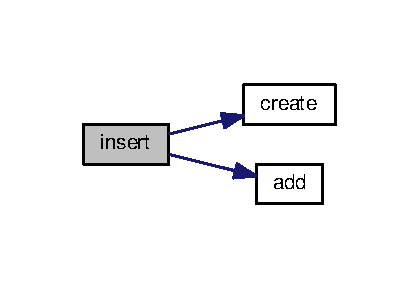
\includegraphics[width=201pt]{Summation_8c_a7f9d39f8cecd6bcb70ada2b9e933eb1e_cgraph}
\end{center}
\end{figure}


\index{Summation.\+c@{Summation.\+c}!main@{main}}
\index{main@{main}!Summation.\+c@{Summation.\+c}}
\subsubsection[{\texorpdfstring{main()}{main()}}]{\setlength{\rightskip}{0pt plus 5cm}void main (
\begin{DoxyParamCaption}
{}
\end{DoxyParamCaption}
)}\hypertarget{Summation_8c_acdef7a1fd863a6d3770c1268cb06add3}{}\label{Summation_8c_acdef7a1fd863a6d3770c1268cb06add3}

\begin{DoxyCode}
22 \{
23     \textcolor{keywordtype}{int} ch;
24  
25     printf(\textcolor{stringliteral}{"\(\backslash\)n OPERATIONS ---"});
26     printf(\textcolor{stringliteral}{"\(\backslash\)n 1] Insert an element into tree"});
27     printf(\textcolor{stringliteral}{"\(\backslash\)n 2] Display the sum of the elements at the same level"});
28     printf(\textcolor{stringliteral}{"\(\backslash\)n 3] Exit "});    
29     \textcolor{keywordflow}{while} (1)
30     \{                        
31         printf(\textcolor{stringliteral}{"\(\backslash\)nEnter your choice : "});
32         scanf(\textcolor{stringliteral}{"%d"}, &ch);
33         \textcolor{keywordflow}{switch} (ch)
34         \{
35         \textcolor{keywordflow}{case} 1:    
36             \hyperlink{Summation_8c_a7f9d39f8cecd6bcb70ada2b9e933eb1e}{insert}();
37             \textcolor{keywordflow}{break};
38         \textcolor{keywordflow}{case} 2: 
39             \hyperlink{Summation_8c_ad43c3812e6d13e0518d9f8b8f463ffcf}{count} = 0;
40             \hyperlink{Summation_8c_ae1e1dde676c120fa6d10f3bb2c14059e}{max} = 0;
41             \hyperlink{Summation_8c_a044c01529821f650d7100142d8788e6b}{computesum}(\hyperlink{Summation_8c_aa6fca9435ac6dc487f22b85aabd703b5}{root});
42             \hyperlink{Summation_8c_a1e5b20fed15743656bb6d2e6a6ea6269}{display}();
43             \textcolor{keywordflow}{break};
44         \textcolor{keywordflow}{case} 3: 
45             exit(0);
46         \textcolor{keywordflow}{default} :     
47             printf(\textcolor{stringliteral}{"Wrong choice, Please enter correct choice  "});
48             \textcolor{keywordflow}{break};    
49         \}
50     \}
51 \}
\end{DoxyCode}


Here is the call graph for this function\+:
\nopagebreak
\begin{figure}[H]
\begin{center}
\leavevmode
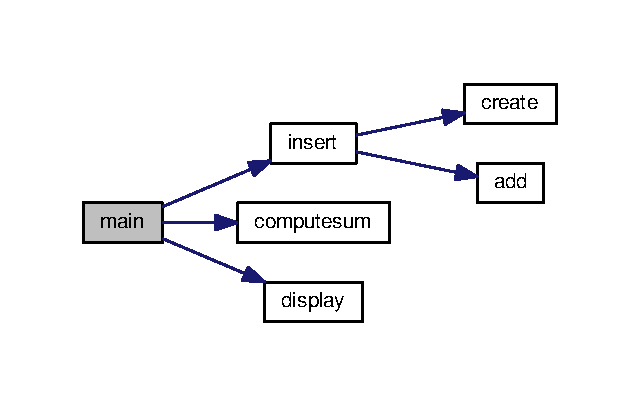
\includegraphics[width=307pt]{Summation_8c_acdef7a1fd863a6d3770c1268cb06add3_cgraph}
\end{center}
\end{figure}




\subsection{Variable Documentation}
\index{Summation.\+c@{Summation.\+c}!count@{count}}
\index{count@{count}!Summation.\+c@{Summation.\+c}}
\subsubsection[{\texorpdfstring{count}{count}}]{\setlength{\rightskip}{0pt plus 5cm}int count = 0}\hypertarget{Summation_8c_ad43c3812e6d13e0518d9f8b8f463ffcf}{}\label{Summation_8c_ad43c3812e6d13e0518d9f8b8f463ffcf}
\index{Summation.\+c@{Summation.\+c}!max@{max}}
\index{max@{max}!Summation.\+c@{Summation.\+c}}
\subsubsection[{\texorpdfstring{max}{max}}]{\setlength{\rightskip}{0pt plus 5cm}int max = 0}\hypertarget{Summation_8c_ae1e1dde676c120fa6d10f3bb2c14059e}{}\label{Summation_8c_ae1e1dde676c120fa6d10f3bb2c14059e}
\index{Summation.\+c@{Summation.\+c}!root@{root}}
\index{root@{root}!Summation.\+c@{Summation.\+c}}
\subsubsection[{\texorpdfstring{root}{root}}]{\setlength{\rightskip}{0pt plus 5cm}struct {\bf btnode}$\ast$ root = N\+U\+LL}\hypertarget{Summation_8c_aa6fca9435ac6dc487f22b85aabd703b5}{}\label{Summation_8c_aa6fca9435ac6dc487f22b85aabd703b5}
\index{Summation.\+c@{Summation.\+c}!sum@{sum}}
\index{sum@{sum}!Summation.\+c@{Summation.\+c}}
\subsubsection[{\texorpdfstring{sum}{sum}}]{\setlength{\rightskip}{0pt plus 5cm}int sum\mbox{[}100\mbox{]} = \{0\}}\hypertarget{Summation_8c_abee91d89f7cb4bbc28d7949ec9d88ea8}{}\label{Summation_8c_abee91d89f7cb4bbc28d7949ec9d88ea8}
\index{Summation.\+c@{Summation.\+c}!temp@{temp}}
\index{temp@{temp}!Summation.\+c@{Summation.\+c}}
\subsubsection[{\texorpdfstring{temp}{temp}}]{\setlength{\rightskip}{0pt plus 5cm}struct {\bf btnode} $\ast$ temp = N\+U\+LL}\hypertarget{Summation_8c_ac0d86a861e85eeb7da1785ac8e3ae769}{}\label{Summation_8c_ac0d86a861e85eeb7da1785ac8e3ae769}

%--- End generated contents ---

% Index
\backmatter
\newpage
\phantomsection
\clearemptydoublepage
\addcontentsline{toc}{chapter}{Index}
\printindex

\end{document}
